%%%%%%%%%%%%%%%%%%%%%%%%%%%%%%%%%%%%%%%%%%%%%%%%%%%%%%%%%%%%%%%%%%%%%
% Mitschrieb vom 03.12.2013                                         %
%%%%%%%%%%%%%%%%%%%%%%%%%%%%%%%%%%%%%%%%%%%%%%%%%%%%%%%%%%%%%%%%%%%%%
\chapter{Fundamentalgruppe und Überlagerungen}
\section{Homotopie von Wegen}
\begin{figure}[ht]
    \centering
    \subfloat[$\gamma_1$ und $\gamma_2$ sind homotop, da man sie 
             \enquote{zueinander verschieben} kann.]{
        \documentclass[varwidth=true, border=2pt]{standalone}

\usepackage{pgfplots}
\usepackage{tikz}

\begin{document}
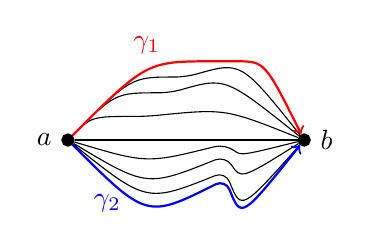
\begin{tikzpicture}
    \tikzstyle{point}=[circle,thick,draw=black,fill=black,inner sep=0pt,minimum width=4pt,minimum height=4pt]
    \node (a)[point,label=180:$a$] at (0,0) {};
    \node (b)[point,label=0:$b$]   at (3, 0) {};
    \draw [rounded corners] (a) .. controls (0.8,0.8) .. (1.5,0.8) .. controls (2.2,1) .. (b);
    \draw [rounded corners] (a) .. controls (0.6,0.6) .. (1.3,0.6) .. controls (2.0,0.8) .. (b);
    \draw [rounded corners] (a) .. controls (0.3,0.3) .. (1.0,0.3) .. controls (2.0,0.4) .. (b);
    \draw [rounded corners] (a) -- (b);
    \draw [rounded corners] (a) .. controls (1,-0.8) .. (2,-0.4) .. controls (2.2,-0.9) .. (b);
    \draw [rounded corners] (a) .. controls (1,-0.6) .. (2,-0.2) .. controls (2.2,-0.5) .. (b);
    \draw [rounded corners] (a) .. controls (1,-0.3) .. (2,-0.05) .. controls (2.2,-0.2) .. (b);
    \draw [rounded corners,->, thick, red] (a) .. controls (1,1) .. (2,1) .. controls (2.5,1) .. (b);
    \draw [rounded corners,->, thick, blue] (a) .. controls (1,-1) .. (2,-0.5) .. controls (2.2,-1) .. (b);
    \node at (1,1.2) [red] {$\gamma_1$};
    \node at (0.5,-0.8) [blue] {$\gamma_2$};
\end{tikzpicture}
\end{document}

        \label{fig:homotope-wege-anschaulich}
    }\hspace{1em}%
    \subfloat[$\gamma_1$ und $\gamma_2$ sind wegen dem Hindernis nicht homotop.]{
        \begin{tikzpicture}
    \tikzstyle{point}=[circle,thick,draw=black,fill=black,inner sep=0pt,minimum width=4pt,minimum height=4pt]
    \node (a)[point,label=180:$a$] at (0,0) {};
    \node (b)[point,label=0:$b$]   at (3, 0) {};
    \draw[orange,pattern color=orange,pattern=north east lines] (1.5,0) circle (0.3cm);
    \draw [rounded corners,->, thick, red] (a) .. controls (1,1) .. (2,1) .. controls (2.5,1) .. (b);
    \draw [rounded corners,->, thick, blue] (a) .. controls (1,-1) .. (2,-0.5) .. controls (2.2,-1) .. (b);
    \node at (1,1.2) [red] {$\gamma_1$};
    \node at (0.5,-0.8) [blue] {$\gamma_2$};
\end{tikzpicture}

        \label{fig:nicht-homotope-wege-anschaulich}
    }
    \label{Formen}
    \caption{Beispiele für Wege $\gamma_1$ und $\gamma_2$}
\end{figure}

\begin{definition}
    Sei $X$ ein topologischer Raum, $a, b \in X$, 
    $\gamma_1, \gamma_2: [0,1] \rightarrow X$ Wege von $a$ nach $b$,
    d.~h. $\gamma_1(0) = \gamma_2(0) = a$, $\gamma_1(1) = \gamma_2(1) = b$

    \begin{enumerate}[label=\alph*)]
        \item $\gamma_1$ und $\gamma_2$ heißen \textbf{homotop}\xindex{homotop}
              ($\gamma_1 \sim \gamma_2$), wenn es eine stetige Abbildung
              \[H(t,0) = \gamma_1(t), H(t,1) = \gamma_2(t) \;\;\; \forall t \in [0,1] =: I \]
              und $H(0,s) = a$ und $H(1,s) = b$ für alle $s \in I$ gibt.

              $H$ heißt \textbf{Homotopie}\xindex{Homotopie} zwischen
              $\gamma_1$ und $\gamma_2$.
        \item $\gamma_s: I \rightarrow X, \gamma_s(t) = H(t,s)$ ist
              Weg in $X$ von $a$ nach $b$ für jedes $s \in I$.
    \end{enumerate}
\end{definition}

\begin{korollar}
    \enquote{Homotop} ist eine Äquivalenzrelation auf der Menge aller
    Wege in $X$ von $a$ nach $b$.
\end{korollar}

\begin{beweis}\leavevmode
    \begin{itemize}
        \item reflexiv: $H(t,s) = \gamma(t)$ für alle $t,s \in I \times I$
        \item symmetrisch: $H'(t,s) = H(t,1-s)$ für alle $t,s \in I \times I$
        \item transitiv: Seien $H'$ bzw. $H''$ Homotopien von $\gamma_1$
              nach $\gamma_2$ bzw. von $\gamma_2$ nach $\gamma_3$.

              Dann sei $H(t,s) := \begin{cases}
              H'(t, 2s)    &\text{falls } 0 \leq s \leq \frac{1}{2}\\
              H''(t, 2s-1) &\text{falls } \frac{1}{2} \leq s \leq 1\end{cases}$

              $\Rightarrow$ $H$ ist stetig und Homotopie von $\gamma_1$ nach 
              $\gamma_2$
    \end{itemize}
    $\qed$
\end{beweis}

\begin{beispiel}
    \begin{enumerate}[label=\arabic*)]
        \item Sei $X = S^1$. $\gamma_1$ und $\gamma_2$ aus 
              Abb.~\ref{fig:circle-two-paths} nicht homöotop.
              \begin{figure}
                \centering
                \documentclass[varwidth=true, border=2pt]{standalone}

\usepackage{pgfplots}
\usepackage{tikz}

\begin{document}
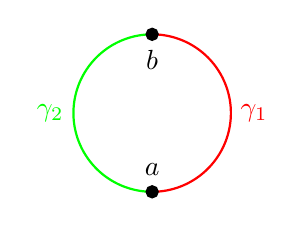
\begin{tikzpicture}
    \tikzstyle{point}=[circle,thick,draw=black,fill=black,inner sep=0pt,minimum width=4pt,minimum height=4pt]
    \draw [red,  thick,domain=90:-90,  samples=100] plot ({cos(\x)}, {sin(\x)});
    \draw [green,thick,domain=-90:-270,samples=100] plot ({cos(\x)}, {sin(\x)});
    \node (a)[point,label=90:$a$] at (0,-1cm) {};
    \node (b)[point,label=-90:$b$] at (0, 1cm) {};

    \node at (1,0) [anchor=180, red] {$\gamma_1$};
    \node at (-1,0) [anchor=0, green] {$\gamma_2$};

\end{tikzpicture}
\end{document}

                \caption{Kreis mit zwei Wegen}
                \label{fig:circle-two-paths}
              \end{figure}
        \item Sei $X = T^2$. $\gamma_1, \gamma_2$ und $\gamma_3$
              aus Abb.~\ref{fig:torus-three-paths} sind paarweise
              nicht homöotop.
              \begin{figure}
                \centering
                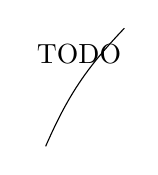
\begin{tikzpicture}
    \path (0,0)  edge [bend angle=10,bend right] node[label=TODO] {} (-1,-1.5);
\end{tikzpicture}

                \caption{Torus mit drei Wegen}
                \label{fig:torus-three-paths}
              \end{figure}
        \item Sei $X = \mdr^2$ und $a=b=(0,0)$. 

              Je zwei Wege im $\mdr^2$ mit Anfangs- und Enpunkt $(0,0)$
              sind homöotop.

              \begin{figure}
                \centering
                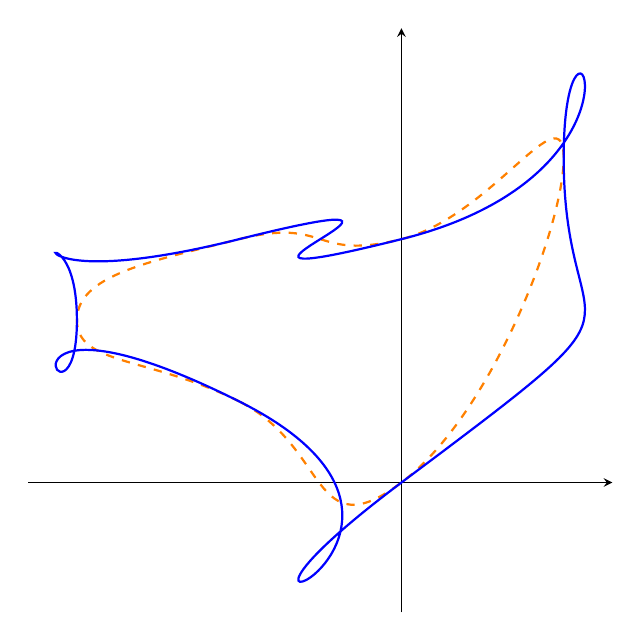
\begin{tikzpicture}
    \begin{axis}[
        legend pos=south west,
        axis x line=middle,
        axis y line=middle,
        %grid = major,
        width=9cm,
        height=9cm,
        grid style={dashed, gray!30},
        xmin=-2,     % start the diagram at this x-coordinate
        xmax= 1,    % end   the diagram at this x-coordinate
        ymin=-1,     % start the diagram at this y-coordinate
        ymax= 5,   % end   the diagram at this y-coordinate
        %axis background/.style={fill=white},
        %xlabel=$x$,
        %ylabel=$y$,
        ticks=none,
        %tick align=outside,
        %minor tick num=-3,
        enlargelimits=true,
        tension=0.08]
        \addplot[mark=none, orange, smooth cycle, thick, tension=1, dashed] coordinates {%
   (0,0) (-1,1) (-2,2) (-1,3) (0, 3) (1, 4)};
        \addplot[mark=none, blue, smooth cycle, thick, tension=3] coordinates {%
   (0,0) (-1,1) (-2,2) (-1,3) (0, 3) (1, 4)};
    \end{axis} 
\end{tikzpicture}

                \caption{Zwei Wege im $\mdr^2$ mit Anfangs- und Enpunkt $(0,0)$}
                \label{fig:torus-three-paths}
              \end{figure}

              Sei $\gamma_0: I \rightarrow \mdr^2$ der konstante Weg
              $\gamma_0(t) = 0 \; \forall t \in I$. Sei
              $\gamma(0) = \gamma(1) = 0$.

              $H(t,s) := (1-s) \gamma(t)$ ist stetig, 
              $H(t,0) = \gamma(t)\; \forall t \in I$ und
              $H(t,1) = 0 \; \forall t \in I$
    \end{enumerate}
\end{beispiel}

% Die Übungsaufgaben sollen ganz am Ende des Kapitels sein.
\clearpage
\section*{Übungsaufgaben}
\addcontentsline{toc}{section}{Übungsaufgaben}

\begin{aufgabe}\label{ub5:aufg1}
    \todo{Todo}
\end{aufgabe}

